\chapter{Benchmarks}
\label{chap:benchmarks}

% arango import: 20s
% orientdb import: 424

In the previous chapters, we have introduced the concept of language switching and the unified algebra. We have implemented three query languages and various optimizations. Next, we will evaluate DortDB and see how we fare compared to other established solutions. We will first examine the viability of our approach on multimodel workloads. Then, we will focus on DortDB as a framework for SQL in JavaScript environments.

All of the experiments were conducted on a machine with a 12-core AMD Ryzen 9 7900 CPU, a 32 GB 6000 MHz RAM, and an SSD.

\section{UniBench}
\label{sec:unibench}

UniBench\cite{zhang2018unibench} is a benchmark designed for evaluating multimodel databases. It provides a data model simulating \textit{social commerce}, a combination of social media and E-commerce. We will use a pre-generated 1 GB dataset, as well as a smaller sample created by selecting data about a hundred customers, which is 5 MB in size. Besides data, the benchmark specifies 10 analytical queries combining relational, document, and graph data models. The queries are described in natural language and need to be rewritten for each tested system, as different multimodel databases use different query languages. The queries used by DortDB are included in appendix \ref{apx:unibench-queries}.

\begin{figure}[!ht]
    \centering
    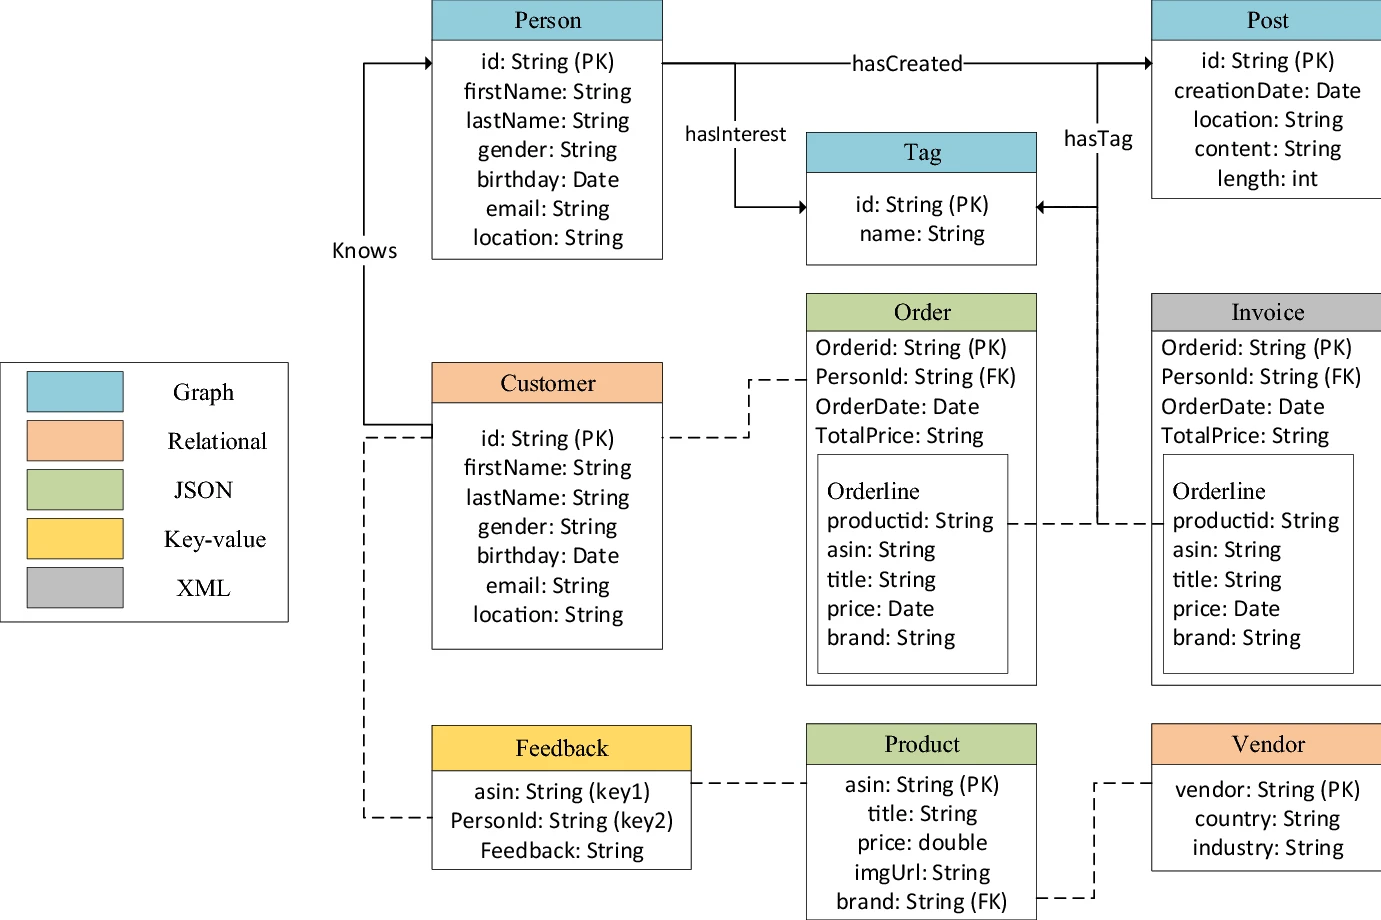
\includegraphics[width=\linewidth]{img/unibench-schema.png}
    \caption{Schema of the UniBench data model\cite{zhang2021holistic}.}
\end{figure}

Part of the UniBench repository are example queries for ArangoDB\footnote{\url{https://arangodb.com/}} and OrientDB\footnote{\url{https://orientdb.dev/}}, as well as scripts for importing data into the database systems. We have used OrientDB version 2.2.16, the same as in the original paper, because the importing mechanisms have changed since, and the provided scripts could not be used otherwise. The importing scripts had to be slightly modified anyway, and we had to configure several indices and vertex properties in the database schema in order for the OrientDB queries to work. The ArangoDB version used was 3.12.5, the latest at the time of writing. There were no issues with either the ArangoDB data import or the ArangoDB queries.

\subsection{Data import}

We have measured the time it takes to import data into the system. In DortDB, the UniBench data was uncompressed from a zip archive, parsed, and stored in memory. Additionally, the data sources were indexed. This was done multiple times and averaged. The ArangoDB and OrientDB measurements come from the provided import scripts, and the data was imported only once.

\begin{listing}[!ht]
\begin{minted}{ts}
db.createIndex(['defaultGraph', 'nodes'], [], ConnectionIndex);
db.createIndex(['defaultGraph', 'nodes'], ['x.id'], MapIndex, {
  mainLang: 'cypher',
  fromItemKey: ['x'],
});
db.createIndex(['defaultGraph', 'edges'], [], ConnectionIndex);
db.createIndex(['customers'], ['id'], MapIndex);
db.createIndex(['products'], ['productId'], MapIndex);
db.createIndex(['products'], ['brand'], MapIndex);
db.createIndex(['products'], ['asin'], MapIndex);
db.createIndex(['feedback'], ['productAsin'], MapIndex);
db.createIndex(['brandProducts'], ['brandName'], MapIndex);
db.createIndex(['brandProducts'], ['productAsin'], MapIndex);
db.createIndex(['vendors'], ['id'], MapIndex);
db.createIndex(['posts'], ['id'], MapIndex);
db.createIndex(['orders'], ['PersonId'], MapIndex);
\end{minted}
\caption{Indices created on DortDB UniBench data sources.}
\end{listing}

\begin{figure}[!ht]
    \centering
    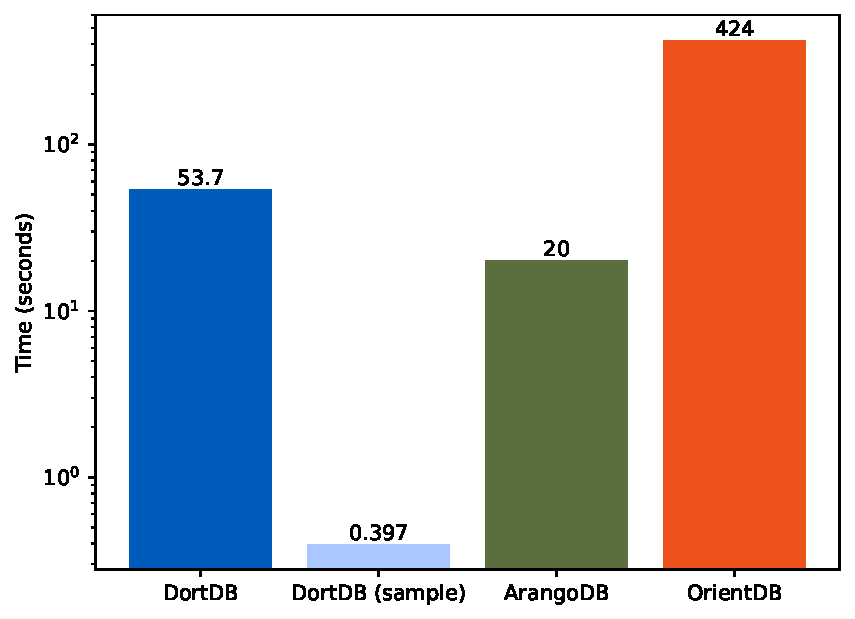
\includegraphics[width=0.6\linewidth]{img/unibench-init.pdf}
    \caption{Processing time for data import.}
    \label{fig:unibench-init}
\end{figure}

The results are displayed in Figure \ref{fig:unibench-init}. Disregarding the sampled dataset, ArangoDB was more than twice as fast as DortDB, even though DortDB did not write anything to disk. One possible explanation is that DortDB runs in a single thread, while ArangoDB is multithreaded. OrientDB data import took around 7 minutes, which is within the realm of expectation.

\subsection{Query performance}

Each query was executed multiple times, and the execution times were averaged. Most of the queries were repeated 10 times, except for DortDB queries that took more than 3 hours or failed. Some of the queries are designed as parametrized, for example, a query that fetches all information available on a certain customer. These parameters were randomized for each execution and taken from a pool provided as part of the dataset.

\begin{figure}[!ht]
    \centering
    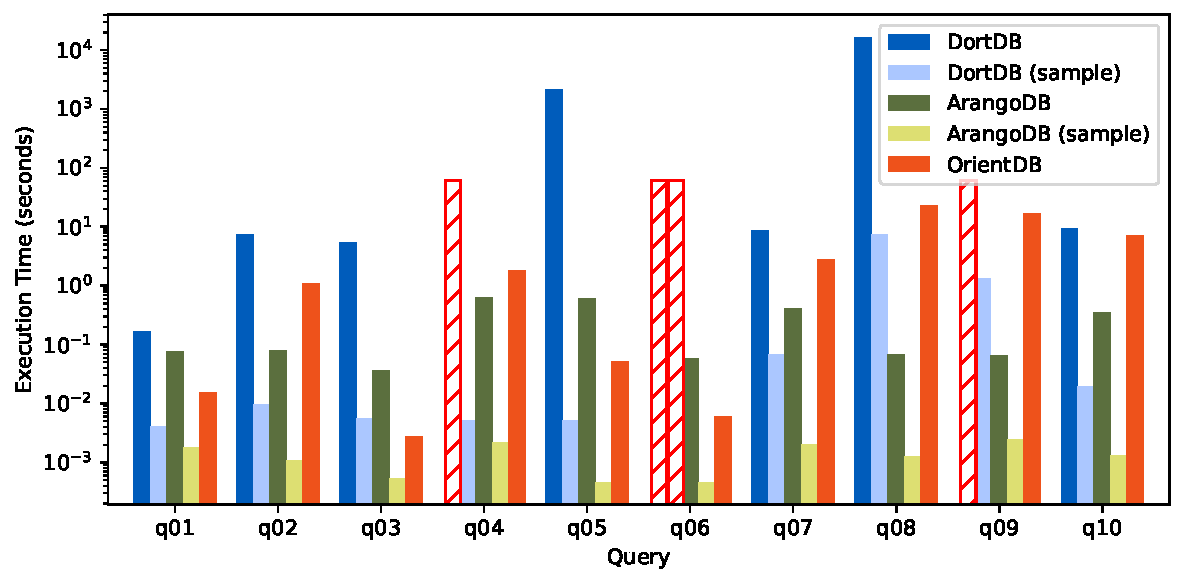
\includegraphics[width=\linewidth]{img/unibench-execution.pdf}
    \caption{Average execution time for each query.}
    \label{fig:unibench-execution}
\end{figure}

The results can be seen in Figure \ref{fig:unibench-execution}. Interestingly enough, OrientDB outperforms ArangoDB in several queries, which contrasts with the measurements in the original paper. On the other hand, DortDB is the slowest, in some cases, more than a hundred times. Three of the DortDB queries failed due to running out of memory. In queries 4 and 6, this is caused by recursive graph traversal. Query 6 ran out of memory even on the small data sample, because its goal was to find the shortest path between two customers, and the randomized customers from the sample were not connected at all. Query 9 does not feature any recursion, and the reasons for its high memory consumption are less immediately recognizable. The query features a large number of logical operators that materialize the whole underlying data stream, such as \texttt{orderBy} or \texttt{treeJoin}. Other databases may avoid this problem by saving intermediary data to disk and using algorithms such as external sorting.

In general, large execution times in DortDB correspond to complex graph traversal and, more markedly, XML tree traversal. The framework currently does not feature any XML tree access optimizations besides the general optimizer rules, nor does it feature any XML indices.

In query 8, the XQuery subquery passes tuple data to SQL as an XML element. We have tested an alternate version of the query without the XML element, and the performance difference was negligible.

On the other hand, DortDB works well with relational data and aggregating queries such as query 10. While it never outperforms any of the competing database systems, we need to remember that it runs in an interpreted language and in a single thread.

\subsection{Query memory usage}

The previous section highlighted a vital problem for in-memory databases: memory consumption. The statistics for DortDB were collected by invoking the garbage collector immediately before the query and comparing the process's memory usage before the query starts and after it finishes. This is by no means a completely accurate reflection of the actual query demands, but it gives us some insight. The garbage collector may be invoked during query if necessary, but as long as there is enough available memory, it will simply continue to be filled. We have observed a query fill the entire memory, and the garbage collector freeing 10 GB of space immediately afterwards.

ArangoDB provides peak memory usage as part of its query statistics. OrientDB does not offer such information and does not participate in the results, which are available in Figure \ref{fig:unibench-memory}.

\begin{figure}[!ht]
    \centering
    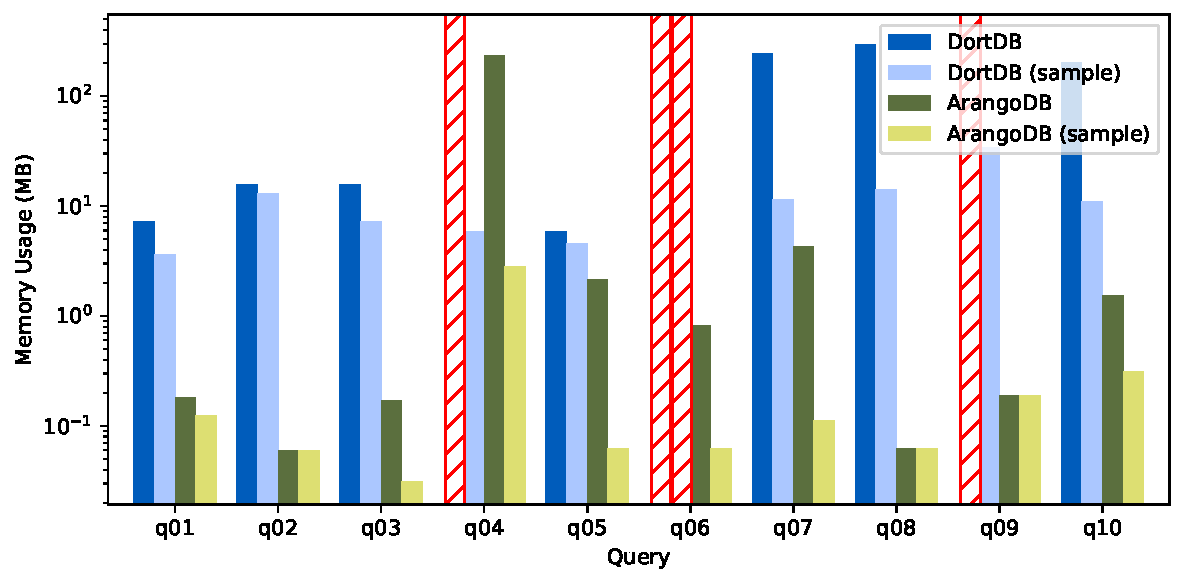
\includegraphics[width=\linewidth]{img/unibench-memory.pdf}
    \caption{Memory usage during each query.}
    \label{fig:unibench-memory}
\end{figure}

We can see that the queries with more materialized operators feature a larger memory usage disparity between DortDB and DortDB (sample). Nevertheless, the difference is never as significant as the difference between dataset sizes. A notable curiosity is query 4, where the sample DortDB memory usage is smaller than in query 3, while on the full dataset, the DortDB ran out of memory. This is because the query iterates over all three-hop common friends of two customers, which are actually not connected in the sample data, and there is therefore nothing to iterate over.

\section{SQL}
\label{sec:sql-benchmarks}

Many benchmarks are available for SQL databases, but the TPC-H\footnote{\url{https://www.tpc.org/tpch/}} is perhaps the best known. It features 22 analytical queries with a moderate to high level of complexity. We have generated data and the queries with an open-source alternative to the official benchmark\footnote{\url{https://github.com/gregrahn/tpch-kit}}. The data was generated with a scale factor of 0.1, resulting in 100 MB of data. The queries were slightly modified for each database in order to adapt to different flavors of SQL. Query 15 was skipped altogether, because it features a \texttt{CREATE VIEW} clause and DortDB does not support either that or \texttt{WITH} common table expressions. The queries are available in appendix \ref{apx:tpch-queries}.

\begin{figure}
    \centering
    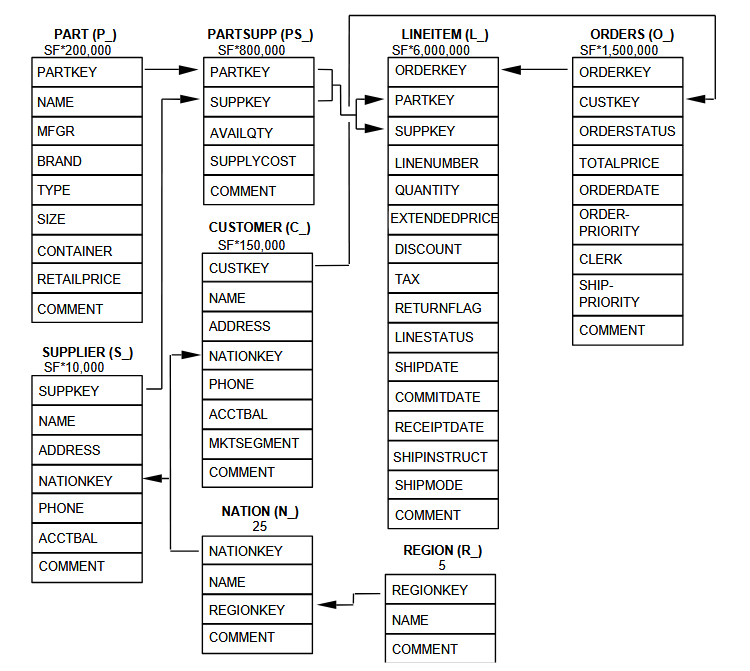
\includegraphics[width=0.7\linewidth]{img/tpch-schema.png}
    \caption{TPC-H benchmark schema. Taken from the TPC-H specification\protect\footnotemark.}
\end{figure}

\footnotetext{\url{https://www.tpc.org/TPC_Documents_Current_Versions/pdf/TPC-H_v3.0.1.pdf}}

\begin{listing}[!ht]
\begin{minted}{ts}
db.createIndex(['customer'], ['custkey'], MapIndex);
db.createIndex(['customer'], ['nationkey'], MapIndex);
db.createIndex(['lineitem'], ['orderkey'], MapIndex);
db.createIndex(['lineitem'], ['partkey'], MapIndex);
db.createIndex(['lineitem'], ['suppkey'], MapIndex);
db.createIndex(['nation'], ['nationkey'], MapIndex);
db.createIndex(['nation'], ['regionkey'], MapIndex);
db.createIndex(['orders'], ['custkey'], MapIndex);
db.createIndex(['orders'], ['orderkey'], MapIndex);
db.createIndex(['part'], ['partkey'], MapIndex);
db.createIndex(['partsupp'], ['partkey'], MapIndex);
db.createIndex(['partsupp'], ['suppkey'], MapIndex);
db.createIndex(['region'], ['regionkey'], MapIndex);
db.createIndex(['supplier'], ['suppkey'], MapIndex);
db.createIndex(['supplier'], ['nationkey'], MapIndex);
\end{minted}
\caption{Indices created for the TPC-H benchmark.}
\end{listing}

We have compared DortDB with two other JavaScript in-memory SQL data\-bases. SQL.js\footnote{\url{https://sql.js.org/}} is SQLite\footnote{\url{https://sqlite.org/}} compiled into WebAssembly, while AlaSQL\footnote{\url{https://github.com/AlaSQL/alasql}} is a rich implementation of SQL with many features. Each query was run up to 10 times, but no longer than an hour. The averaged results are in Figure \ref{fig:tpch-execution}.

\begin{figure}[!ht]
    \centering
    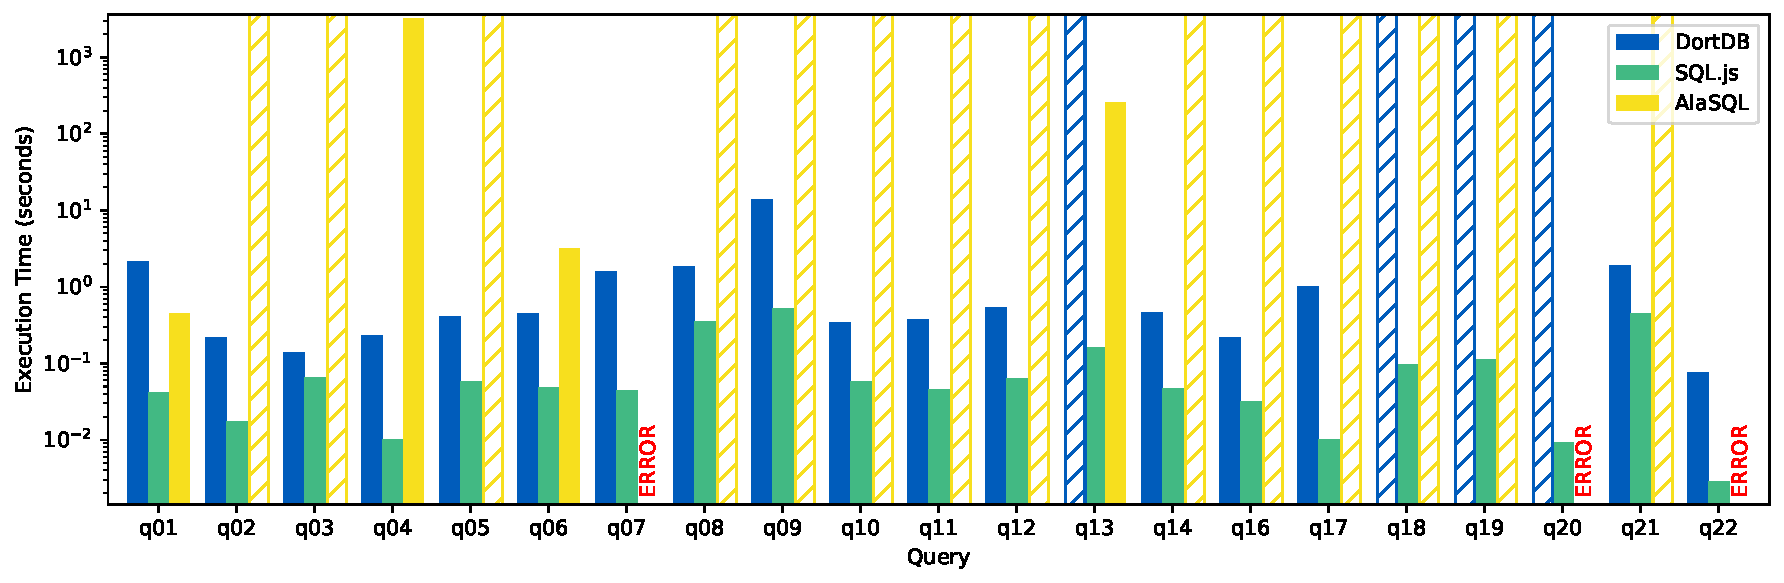
\includegraphics[width=\linewidth]{img/tpch-execution.pdf}
    \caption{Average execution time for each query.}
    \label{fig:tpch-execution}
\end{figure}

It comes as no surprise that SQL.js achieved the best execution times. It runs in native code, and its query optimizer is very powerful, owing to more than 20 years of development. Compared to that, AlaSQL timed out most of the queries and crashed on three. According to its GitHub wiki, it does not have a query optimizer per se, but it preemptively indexes tables before joining, and it tries to push down \texttt{WHERE} conditions before joins. This, unfortunately, does not fare that well when faced with more complex queries. When the queries are simple, like query 1, which focuses on aggregating multiple columns at once, AlaSQL can outperform DortDB thanks to its precompiled queries. Instead of executing a plan in the form of a tree, AlaSQL compiles it into a single function as a concatenation of source code.

DortDB managed most of the queries quite well, timing out on four. Query 13 contains a \texttt{LIKE} comparison with three \texttt{\%} wildcards. Queries 18 and 20 contain complex \texttt{IN} operators, which are currently not optimized. Finally, query 19 tests the optimization of \texttt{OR} conditions, which is also not implemented.